\chapter{Introduction}
Huge influence of computers in society has made smart devices, an important part of our lives. Availability and affordability of such devices motivated us to use them in our day-to-day living. The list of smart devices includes personal automatic and semi-automatic robots which are also playing a major role in our household. For an instance, Roomba \cite{8} is an autonomous robotic vacuum cleaners that automatically cleans the floor and goes to its charging station without human interaction.

Interaction with smart devices has still been mostly through displays, keyboards, mouse and touch interfaces. These devices have grown to be familiar but inherently limit the speed and naturalness with which we can interact with the computer.  Usage of robots for domestic and industrial purposes has been continuously increasing. Thus in recent years, there has been a tremendous push in research toward an intuitive and easy communication with the robot through speech, gestures and facial expressions.

Tremendous progress had been made in speech recognition and several commercially successful speech interfaces are available. However, speech recognition systems have certain limitations such as misinterpretation due to various accents and background noise interference. It may not be able to differentiate between your speech, other people talking and other ambient noise, leading to transcription mix-ups and errors.

Furthermore, there has been an increased interest in recent years in trying to introduce other human-to-human communication modalities into HRI. This includes a class of techniques based on the movement of the human arm and hand, or hand gestures. The use of hand gestures provides an attractive alternative for Human-robot interaction than the conventional cumbersome devices.

\begin{figure}
	[h] \centering 
	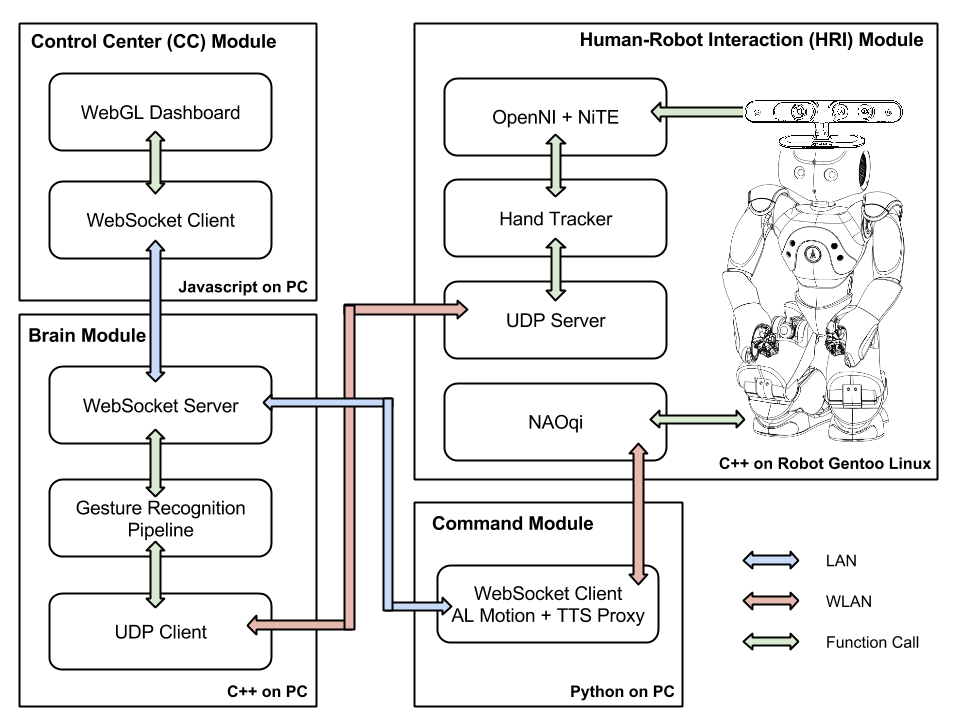
\includegraphics[height=11cm]{figures/content/hri-architecture.png} \caption{HRI Architecture} \label{fg:hri:architecture} 
\end{figure}
